\documentclass[12pt]{beamer}
\usepackage[utf8]{inputenc}
\usepackage[spanish]{babel}
%\usepackage[dvips]{epsfig}
\usepackage{graphics}
\usepackage{svg}
\usepackage{url}
\usepackage{ulem}
\usepackage{beamerthemesplit}
\usepackage{color}
\usepackage{hyperref}
\usepackage{wrapfig}
\usetheme{CambridgeUS}
\setbeamercovered{transparent}

\let\Oldframetitle\frametitle
\renewcommand{\frametitle}[1]{\vspace{0.2cm}\begin{huge}#1\end{huge}\\}
\let\Oldframesubtitle\framesubtitle
\renewcommand{\framesubtitle}[1]{\vspace{0.4cm} \hspace{0.4cm}\begin{large}#1\end{large}\\}

\title{User identification with username and password in structured P2P networks}
\subtitle{}
\author[R. Fernández]{Rodrigo Fernández \\ \small{\texttt{rfernand@inf.utfsm.cl}}}
\institute[]{Universidad Técnica Federico Santa María}
\titlegraphic{
\includegraphics[height=1cm]{img/logo}}
\date{\today}

\begin{document}
  \bibliographystyle{plain}

  \frame{\titlepage}
  \frame{\tableofcontents}

  \section{General formulation of the problem and thesis proposal}
  \subsection{Context and Motivation}

  \begin{frame}
  \frametitle{P2P Networks}
  \framesubtitle{They can be used for}
  
  \begin{table}
  \begin{tabular}{p{7cm}p{3cm}}
  \begin{itemize}
    \item Storage and file sharing
    \item Email
    \item Money (heard about bitcoin?)
    \item and a lot more!
  \end{itemize}
  &
  \vspace{1.5cm}
  %\includegraphics[width=4cm]{../../presentacion/img/p2p-unstructured}\\
  \end{tabular}
  \end{table}
  \end{frame}

    \begin{frame}
    \frametitle{P2P Networks Properties}
    \begin{table}
    \begin{tabular}{p{7cm}p{3cm}}
    \begin{itemize}
      \item Scalable
      \item Decentralized
      \item Self-maintained
      \item Robust
    \end{itemize}
    &
    \vspace{1.5cm}
    \includegraphics[width=4cm]{../../presentacion/img/p2p-unstructured}\\
    \end{tabular}
    \end{table}
    \end{frame}
    
    \begin{frame}
    \frametitle{P2P Networks Overlay structure}
    \begin{table}
    \begin{tabular}{p{7cm}p{3cm}}
    \begin{itemize}
        \item Structured networks (CAN, CHORD, Pastry)
        \item Unstructured networks (Gnutella, Bittorrent)
    \end{itemize}
    &
    \vspace{1.5cm}
    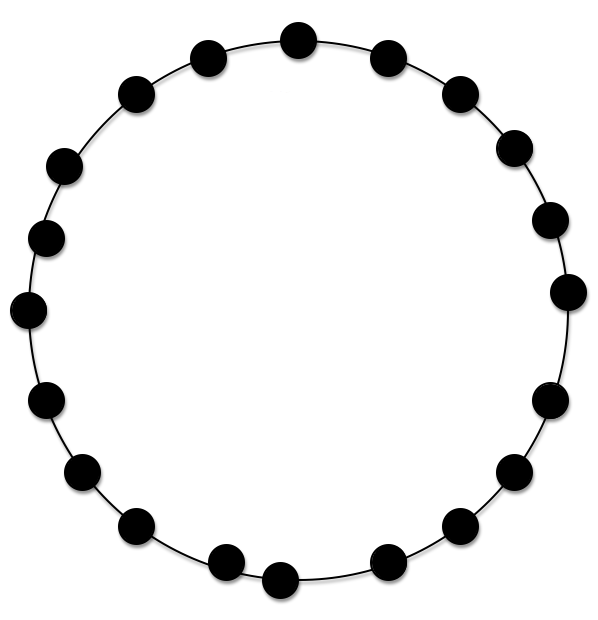
\includegraphics[width=4cm]{../../presentacion/img/p2p-structured}\\
    \end{tabular}
    \end{table}
    \end{frame}

    \begin{frame}
    \frametitle{P2P Networks}
    \framesubtitle{Unstructured networks}
    \begin{table}
    \begin{tabular}{p{7cm}p{3cm}}
    \begin{itemize}
        \item Usually organized as a hierarchical/plain graph.
        \item Search is costly and can result in false negatives.
        \item Can achieve certain grade of node anonymity. 
    \end{itemize}
    &
    \vspace{1.5cm}
    \includegraphics[width=4cm]{../../presentacion/img/p2p-unstructured}\\
    \end{tabular}
    \end{table}
    \end{frame}

    \begin{frame}
    \frametitle{P2P Networks}
    \framesubtitle{Structured networks}
    \begin{table}
    \begin{tabular}{p{7cm}p{3cm}}
    \begin{itemize}
        \item Strong topology structure, usually ring or mesh based.
        \item More efficient search, without false negatives.
        %\item Specific routing algorithm
    \end{itemize}
    &
    \vspace{1.5cm}
    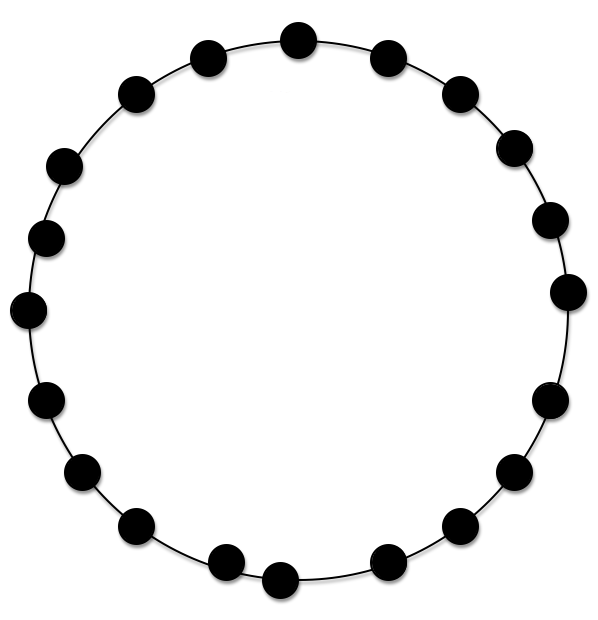
\includegraphics[width=4cm]{../../presentacion/img/p2p-structured}\\
    \end{tabular}
    \end{table}
    \end{frame}

    \begin{frame}
    \frametitle{P2P Networks}
    \framesubtitle{Structured network example: Pastry}
    \begin{table}
    \begin{tabular}{p{6cm}p{4cm}}
    \begin{itemize}
        \item Routing algorithm based on SHA-1
        \item Each node maintains a routing table, leafset and a neighbor set.
        \item Data search reaches O(log(N)) nodes
    \end{itemize}
    &
    \vspace{0.5cm}
    %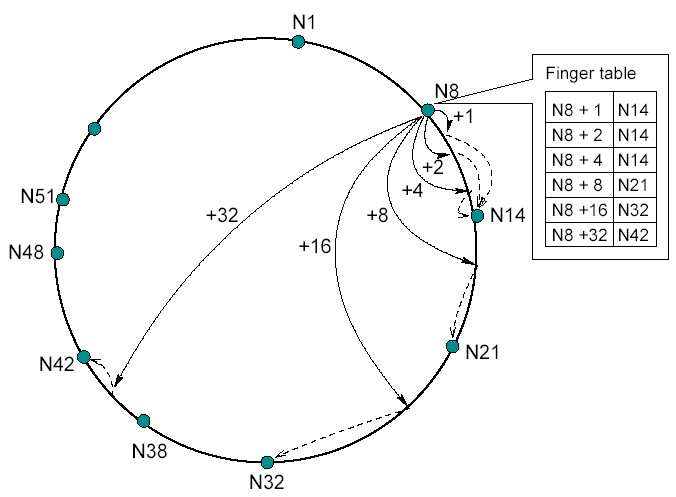
\includegraphics[width=8cm]{../../presentacion/img/chord-search}\\
    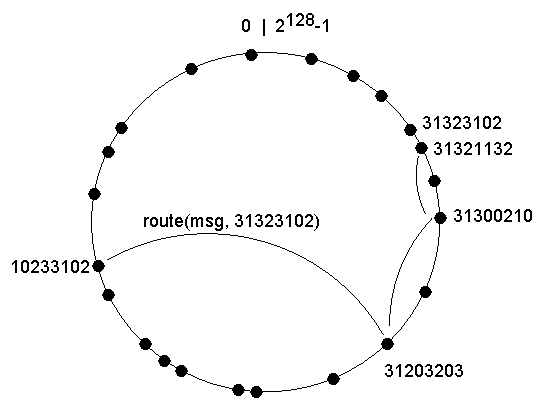
\includegraphics[width=4cm]{../../img/pastryrouting}\\
    \end{tabular}
    \end{table}
    \end{frame}

  \subsection{Problem statement}
  % problem for other solutions- multiple devices per user
  \begin{frame}
  \frametitle{Complex systems needs a way to identify an user...}
  \framesubtitle{In short:}
  \begin{table}
  \begin{tabular}{p{7cm}p{3cm}}
  \begin{itemize}
    \item Many \textbf{complex systems} require authenticated users to work.
    \item Most of the users has \textbf{more than one device}, so identification through
      multiple devices is needed.
    \item \textbf{User are accustomed} to username/password solutions.
  \end{itemize}
  &
  \vspace{1.5cm}
  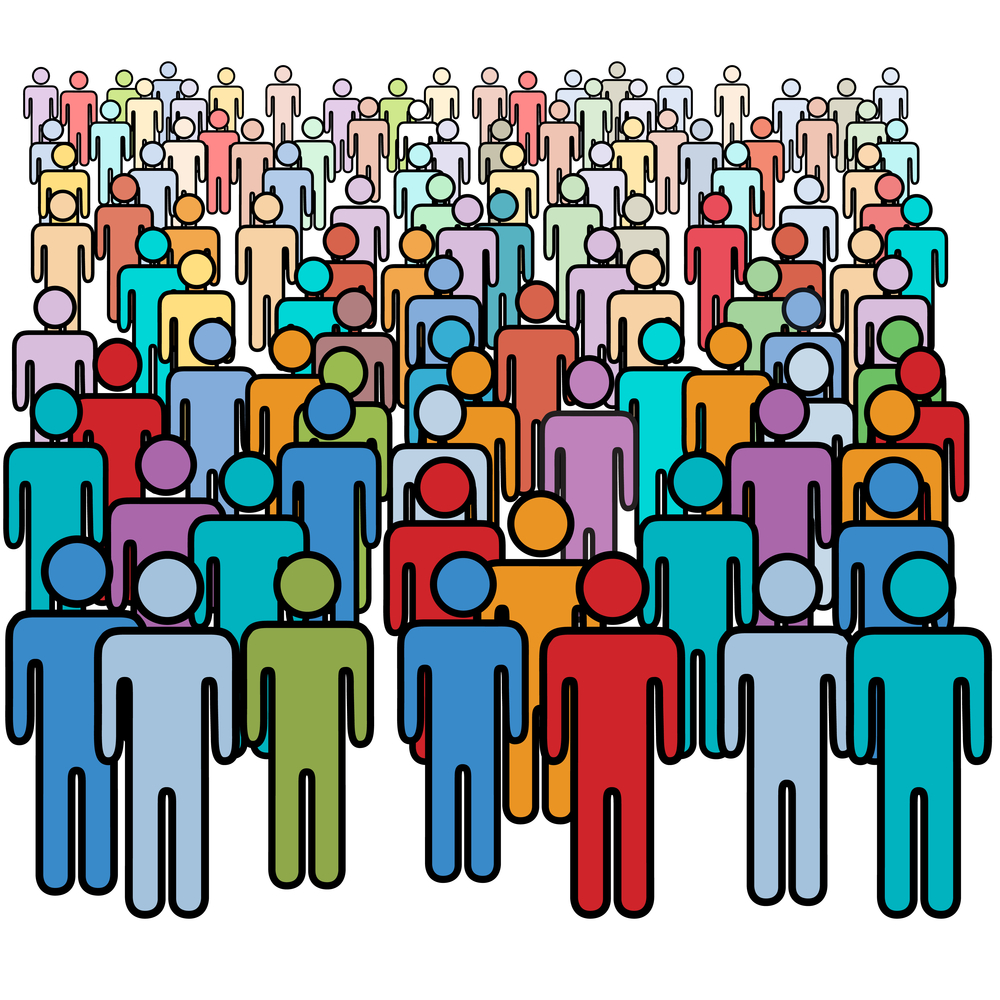
\includegraphics[width=4cm]{../../presentacion/img/users}\\
  \end{tabular}
  \end{table}
  \end{frame}
  
  
  \begin{frame}
  \frametitle{P2P Identification Schemes}
  \framesubtitle{Options?}
  
    Decentralized schemes distributes the task of public key auth to all
    participants.
  \begin{table}
  \begin{tabular}{p{7cm}p{3cm}}
  \begin{itemize}
    \item PGP-like scheme\\ Creates web of trust to auth public keys based on
      their acquaintances opinions.
    \item Quorum-based scheme\\ Multiple independent participants replicate
      public keys.
    \item Username/Password scheme
  \end{itemize}
  &
  \vspace{1.5cm}
  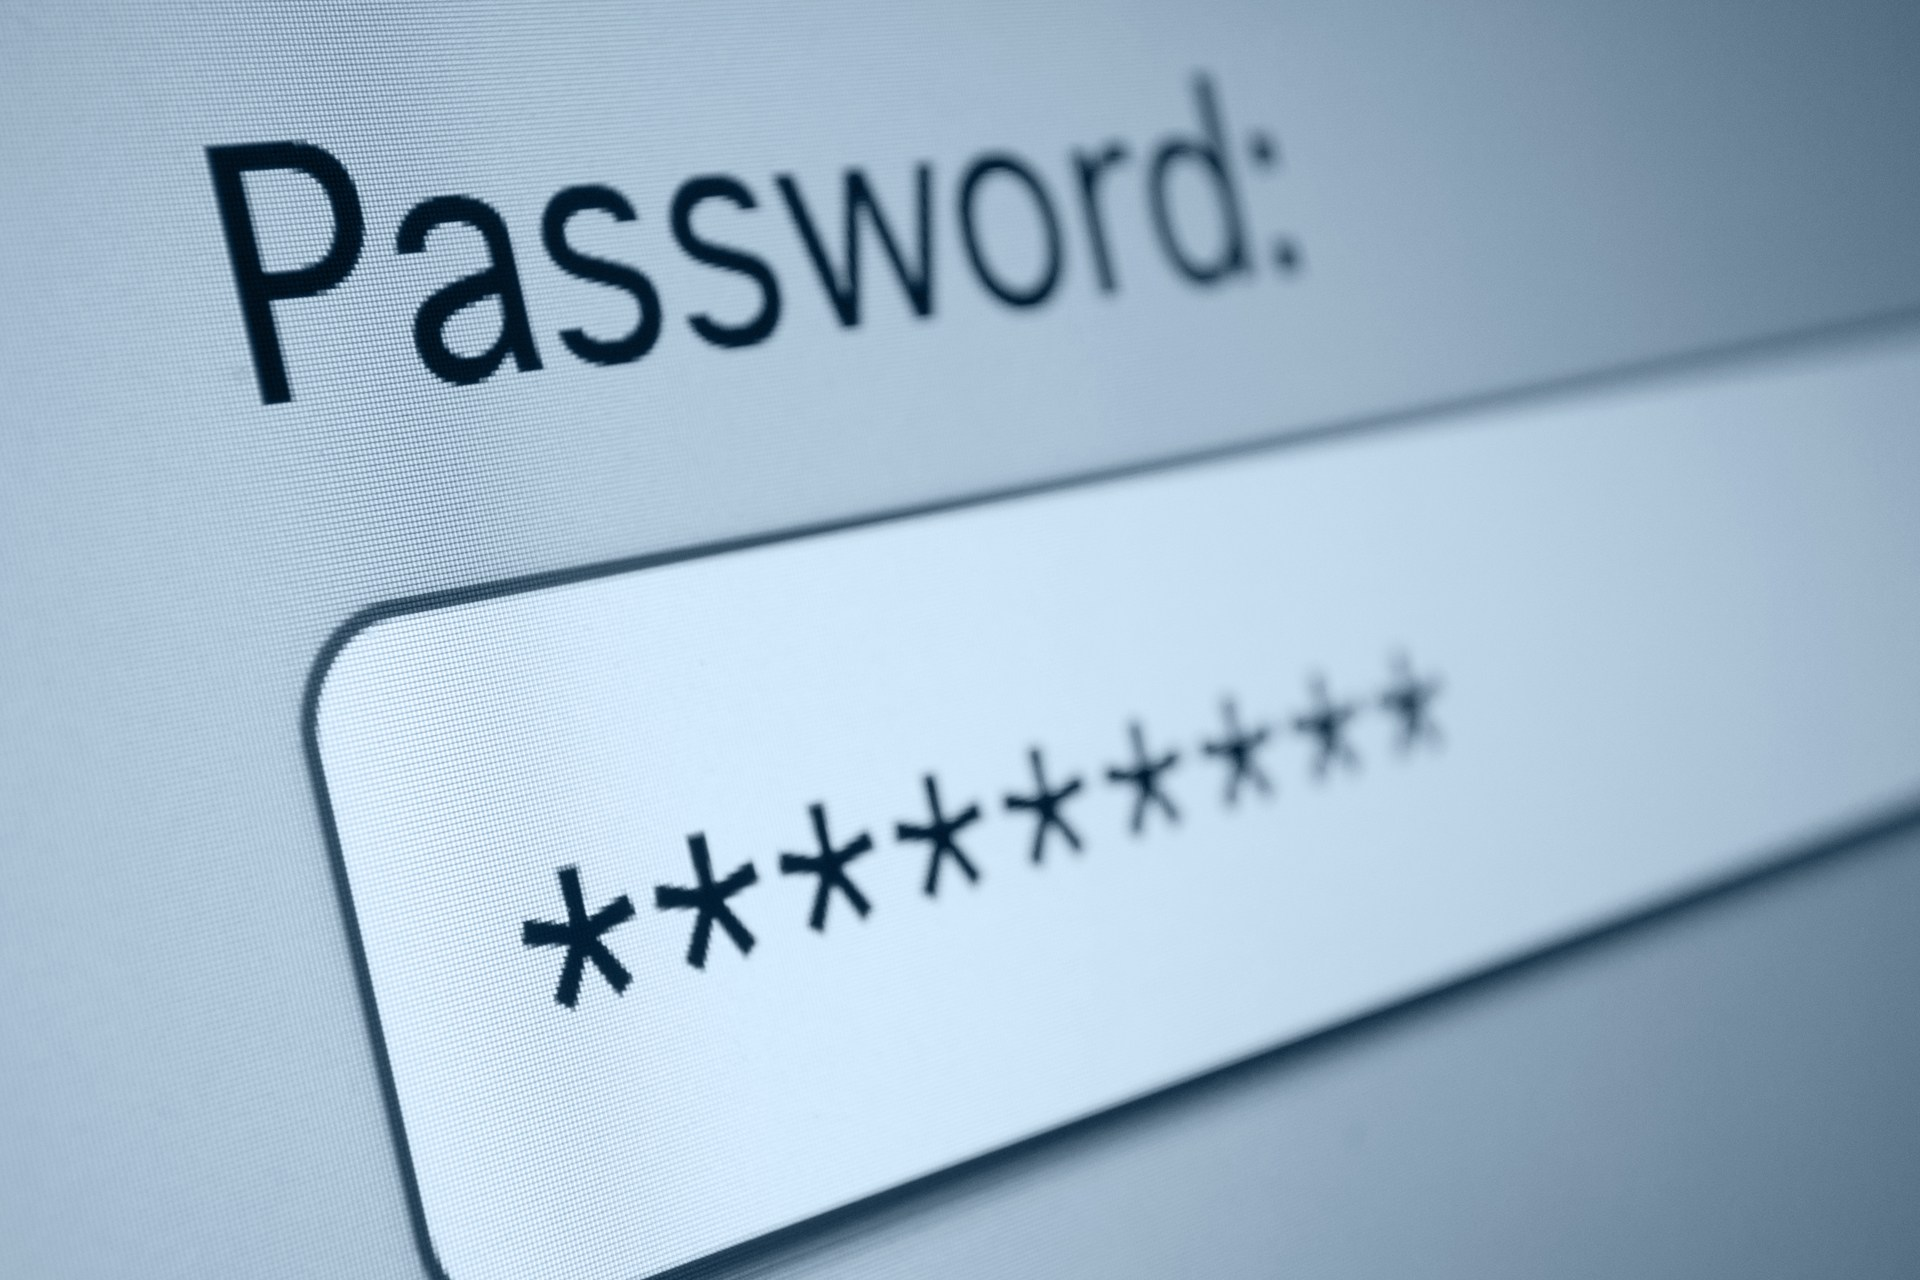
\includegraphics[width=4cm]{../../presentacion/img/password}\\
  \end{tabular}
  \end{table}
  \end{frame}


  \begin{frame}
  \frametitle{Peerson proposal}
  \center
  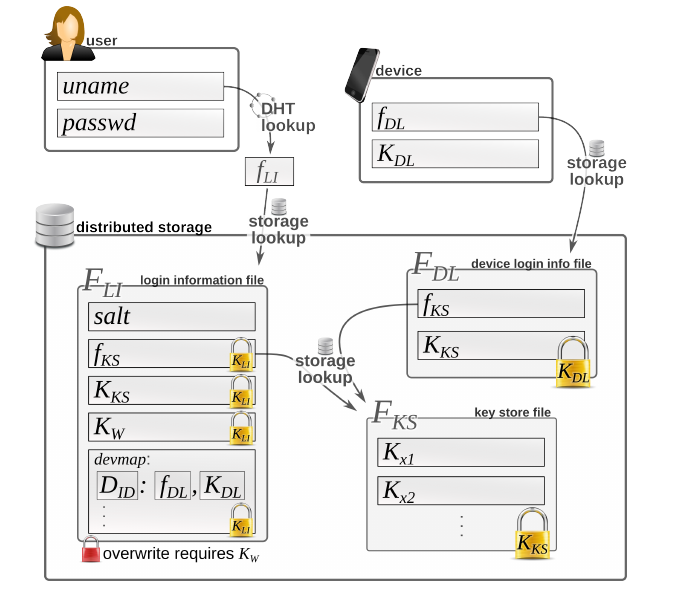
\includegraphics[height=0.9\textheight]{../../../img/password_peerson}\\
  
  \end{frame}

  \begin{frame}
  \frametitle{Peerson proposal}
  \framesubtitle{(simplified version)} 
  \center
  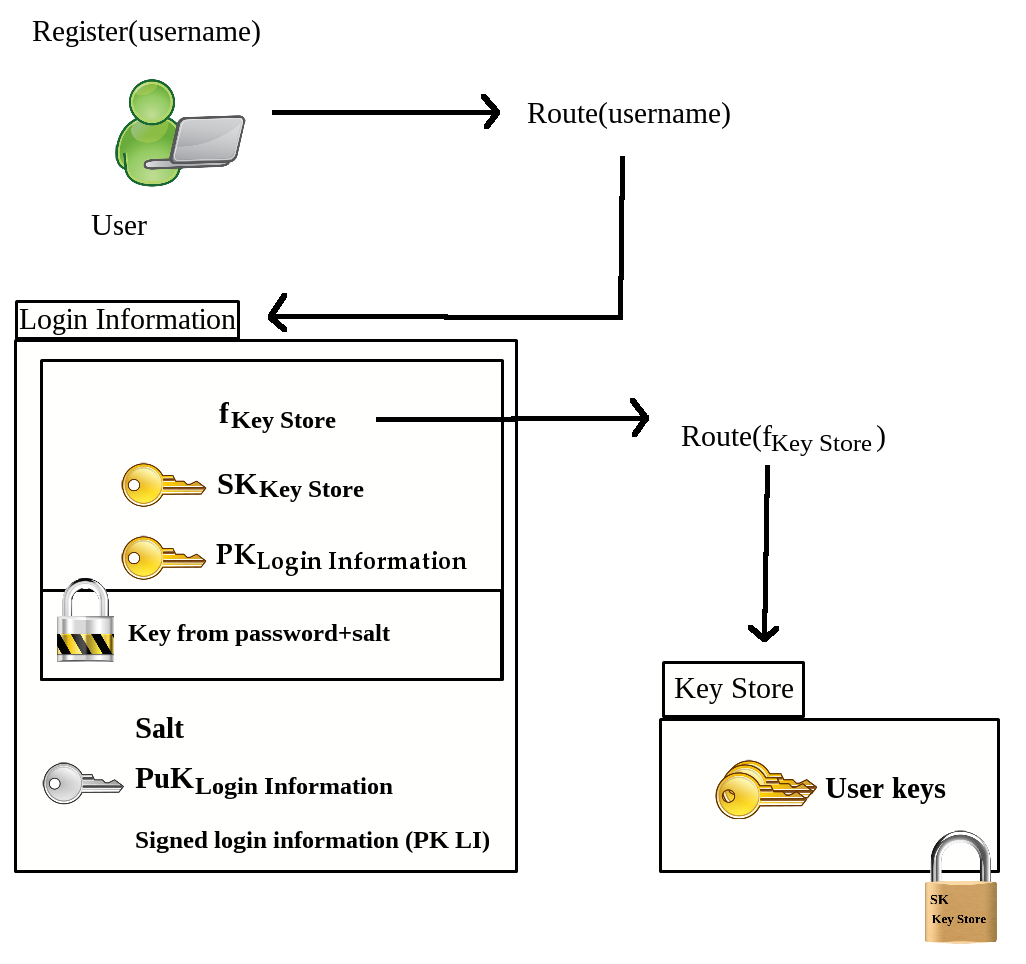
\includegraphics[height=0.7\textheight]{../../../img/password_peerson_alternative}\\
  \end{frame}

  \begin{frame}
  \frametitle{Peerson proposal}
  \framesubtitle{Protocols}

  \begin{enumerate}
    \item User registration
    \item User sign in
    \item Logout
    \item Password change
    \item Password recovery
  \end{enumerate}
  \end{frame}

  \begin{frame}
  \frametitle{Peerson proposal problem...}
  \framesubtitle{It only works in a ``perfect'' world}

  \begin{enumerate}
    \item In reality there are byzantine nodes
    \item How to ensure that a node is telling the truth?
    \item Resilience against Sybil attacks?
  \end{enumerate}
  \end{frame}
  
  \begin{frame}
  \frametitle{Trust in P2P networks}
  \begin{table}
  \begin{tabular}{p{10cm}}
  \begin{enumerate}
      \item To deliver a valuable service in P2P applications, it
  is important to trust that the participants will act as requested.
      \item We need to be sure that other peers will forward
  messages, and that the designated peers will indeed save the information
  correctly so that operations can be successful.
  \end{enumerate}
  \end{tabular}
  \end{table}
  \end{frame}
  
  \begin{frame}
  \frametitle{Trust in P2P networks}
  \framesubtitle{Building Trust}
  %Consequently, the quality of service of applications may
  %be deteriorated due to message overhead or data loss.
  \begin{table}
  \begin{tabular}{p{10cm}}
  \begin{enumerate}
      \item Complex since a P2P network includes untrusted nodes from an open environment.
      \item Untrusted nodes may be faulty, malicious, and act together to attack the network.
  \end{enumerate}
  \end{tabular}
  \end{table}
  \end{frame}

  \begin{frame}
  \frametitle{Trust in P2P networks}
  \framesubtitle{Byzantine nodes}
  \begin{table}
  \begin{tabular}{p{7cm}p{3cm}}
  Are all nodes that not behave as expected
  %Multiples causes: connection problems, viruses, modified software, etc.\\
  %\b{\*Nobody can be trusted}
  \begin{enumerate}
      \item Faulty nodes
      \item Malicious nodes
      \item Infected nodes
  \end{enumerate}
    A peer is honest only if the peers executes the protocol faithfully;
    otherwise, the peer is faulty.
  &
  \vspace{1.5cm}
  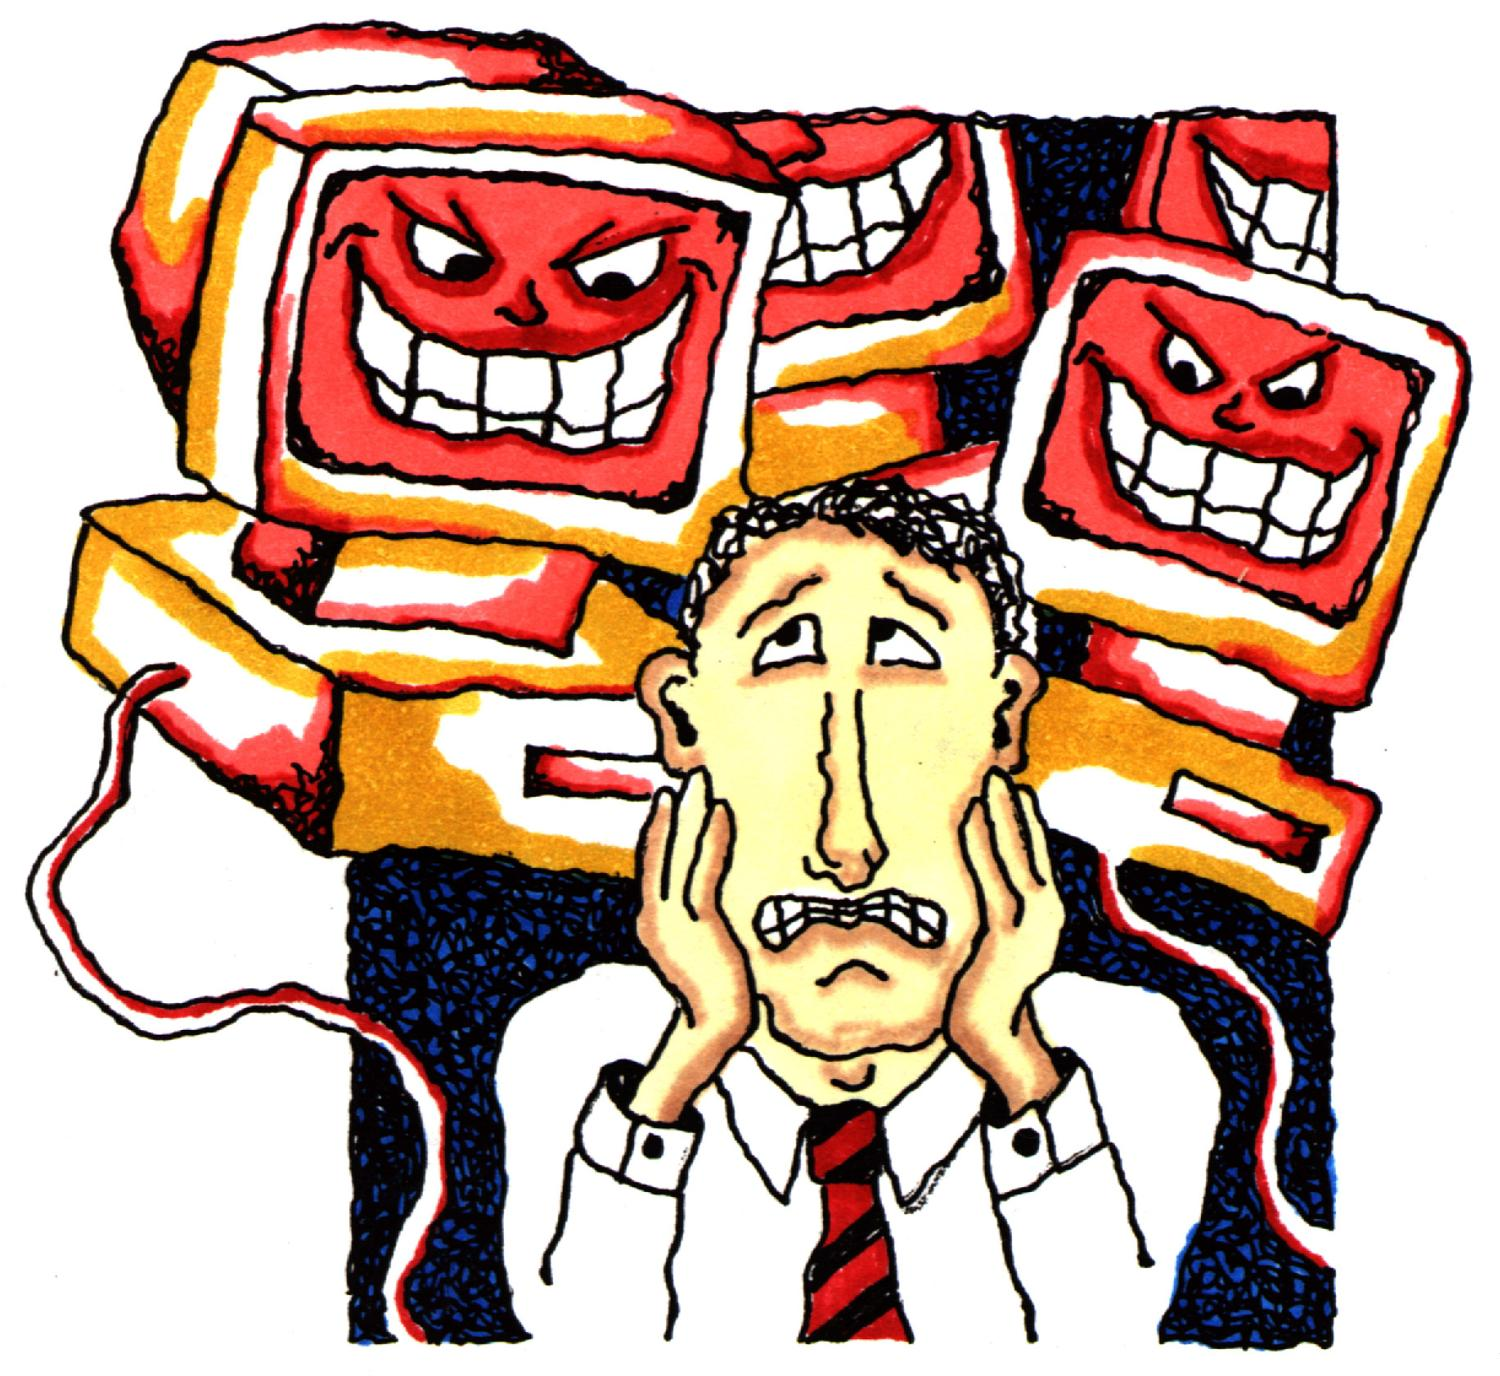
\includegraphics[width=4cm]{../../presentacion/img/malicious}\\
  \end{tabular}
  \end{table}
  \end{frame}
  
  \begin{frame}
  \frametitle{Trust in P2P networks}
  \framesubtitle{How to detect byzantine nodes?}
  %Consequently, the quality of service of applications may
  %be deteriorated due to message overhead or data loss.
  \begin{table}
  \begin{tabular}{p{7cm}p{3cm}}
  \begin{enumerate}
      \item{Reputation systems:} Assess the past history of a
  peer by gathering feedback from nodes with previous interactions with this
  peer.
      \item{Accountability:} Detects and exposes faulty nodes by
  creating non-repudiable records of every node’s actions.
  \end{enumerate}
  &
  \vspace{1.5cm}
  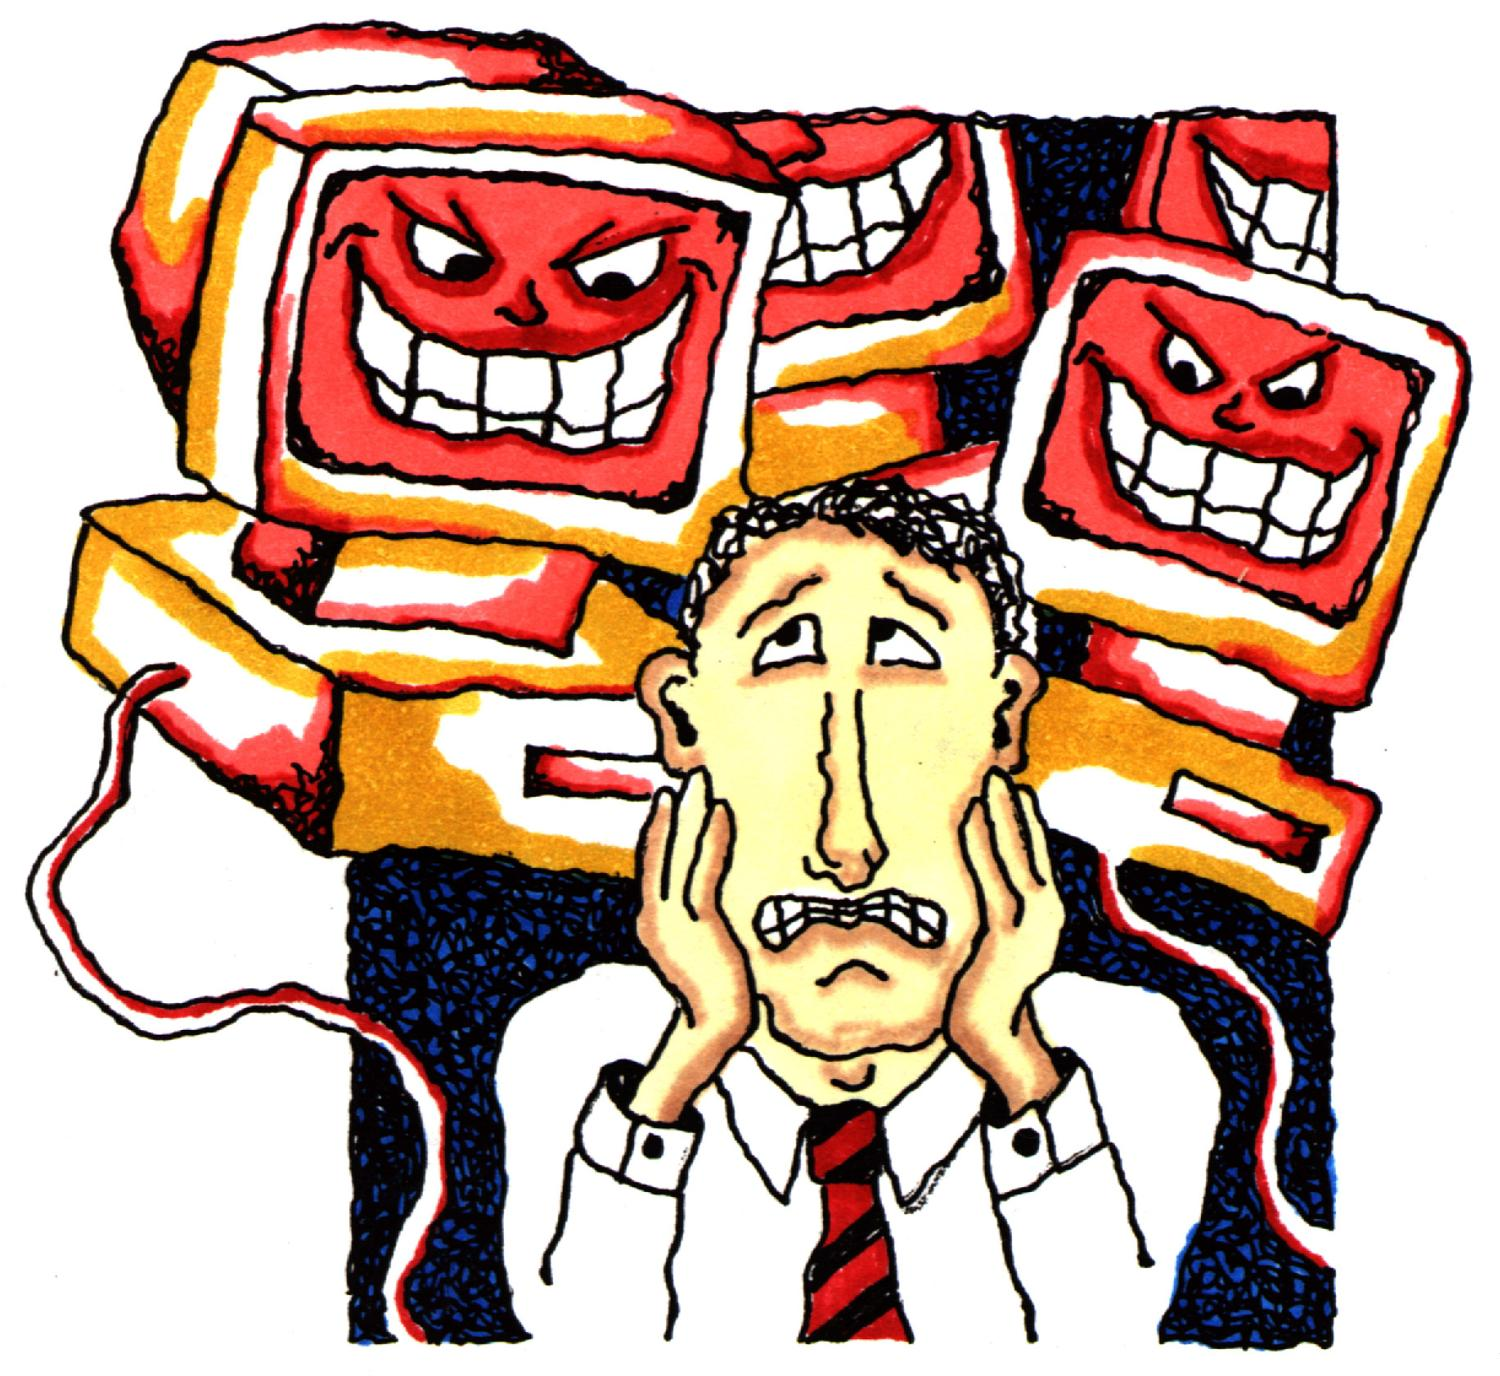
\includegraphics[width=4cm]{../../presentacion/img/malicious}\\
  \end{tabular}
  \end{table}
  \end{frame}

  \begin{frame}
  \frametitle{Reputation systems}
  \framesubtitle{CORPS Trust model}
  %Consequently, the quality of service of applications may
  %be deteriorated due to message overhead or data loss.
  \begin{table}
  \begin{tabular}{p{11cm}}
    \begin{enumerate}
      \item Every node $X$ has an associated reputation value $R(X)$
      which represents the probability that $X$ is an honest node.
      \item $R(X)$ is computed using the recommendations emitted
      by nodes that have completed a transaction with $X$. Bad
      recommendations have a stronger effect on $R(X)$ than
      good ones. It should be more difficult for node to
      increase its reputation value than to decrease it.
      \item For every node $X$, $R(X)$ is highly available in the DHT.
    \end{enumerate}
  \end{tabular}
  \end{table}
  \end{frame}
  
  
  \begin{frame}
  \frametitle{Byzantine node tolerance}
  \begin{table}
  \begin{tabular}{p{7cm}p{3cm}}
    P2P networks can achieve byzantine fault tolerance under $1/3$ byzantine
    peers\\

    \\Group agreement:
    The goal is to obtain at least $\frac{L}{2} + 1$ identical answers from a
group of $L$ nodes.
  &
  \vspace{1.5cm}
  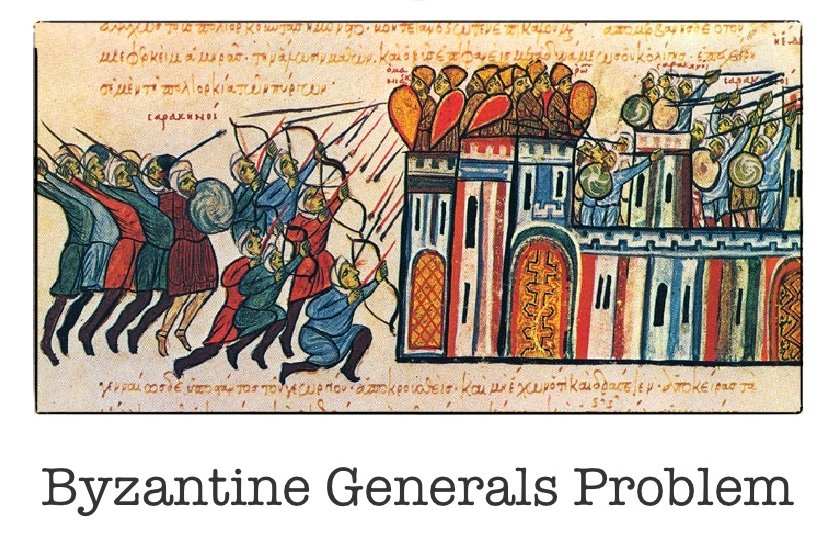
\includegraphics[width=4cm]{../../presentacion/img/bizantine_generals_problem}\\
  \end{tabular}
  \end{table}
  \end{frame}


  %intro of p2p networks


  % identities in P2P networks
  
    % examples



  \subsection{Thesis proposal}
    \begin{frame}
    \frametitle{Thesis proposal}
    \begin{itemize}
      \item Propose and evaluate a new user identification system that can work
in the presence of byzantine nodes in real life scenarios.
    \end{itemize}
    \end{frame}
  %
  %%Before developing an P2P system with the desired functionalities, an adequate
  %%system architecture is needed. We will thoroughly evaluate a new user
  %%identification system that can work in the presence of bizantine nodes, with
  %%the hopes to reach the desirable functionalities with a minimum probability of
  %%failure, to ensure the security of the system in real life scenarios.

  \subsubsection{System architecture}
  % structured p2p and dht based
  % trust management
  % trust-secured protocols
  % criptography schemes

  \section{Working Hypothesis}
    \begin{frame}
    \frametitle{Working Hypothesis}
    %\framesubtitle{Main Goals}
      \begin{itemize}
          \item It is assumed that the use of a reputation system and trusted nodes
            management mitigates the effectivity of malicious nodes on identity
            usurpation attacks.
          \item It is assumed that encryption schemes available today are
            sufficient to secure the user's private data in the P2P networks.
      \end{itemize}
    \end{frame}

  \section{Goals}
  \subsection{Main Goals}
    \begin{frame}
    \frametitle{Goals}
    \framesubtitle{Main Goals}
    The implementation of a secure \textit{username/password} based user identification scheme in structured P2P
    networks using:
    \begin{itemize}
      \item  Secure routing
      \item  Node trust management 
      \item  Encryption schemes
    \end{itemize}
    %\begin{enumerate}
    %    \item Have a minimal possibility of error in the identification process.
    %    \item Use a layer developed scheme that can easily adapt to most commonly
    %          used P2P networks.
    %\end{enumerate}
    \end{frame}

  \subsection{Specifics Goals}
    \begin{frame}
    \frametitle{Goals}
    \framesubtitle{Specifics Goals}
    \begin{itemize}
      \item Study the possibility of password recovery mechanisms.
      \item Study and use trust management to maintain a
            secure layer inside the P2P network.
      \item Use byzantine tolerant algorithms to verify and maintain the
            system consistency in the presence of malicious nodes.
      \item Study and use secure routing, search and storage mechanisms in
            structured P2P networks.
    \end{itemize}
    \end{frame}

  \section{Results}
  \subsection{Contributions and Expected Results}
    \begin{frame}
    \frametitle{Results}
    \framesubtitle{Contributions and Expected Results}
      \begin{itemize}
          \item Design of a secure and modern user identification system for
                structured P2P networks.
          \item Generate a base system to develop complex projects in P2P networks.
          \item Reassure that P2P distributed systems have the capabilities to offer
                complex and high level services.
          \item Paper publication.
                %to be sent to a distributed systems
                %publisher. The paper will show the results of the user identification system
                %designed in this project.
      \end{itemize}
    \end{frame}

  \subsection{Validation procedures}
    \begin{frame}
    \frametitle{Results}
    \framesubtitle{Validation procedures}
    \begin{table}
    \begin{tabular}{p{7cm}p{3cm}}
      %P2P networks presents a big difficulty to be tested in a real environment
      %because of the high number of nodes needed to try it out.
      %Therefore, instead of going after an empiric validation of the proposed
      %identification system, only a  theoretical evaluation will be presented.
      %The proposed system will be compared with the other systems available at
      %the moment with a thoroughly analysis of the security of the algorithm used.
      %
      %Taking that in consideration, the theoretical evaluation will be focused in:
      %
      \begin{itemize}
          \item Proving that the system will have a minimal probability of error.
          \item Proving that the system will  maintain his consistency in networks with at most 30\% of byzantine nodes. 
      \end{itemize}
    &
    \vspace{1.5cm}
    %\includegraphics[width=4cm]{img/p2p-unstructured}\\
    \end{tabular}
    \end{table}
    \end{frame}

  \section{Bibliography}
  \bibliography{../../../bib/article,../../../bib/paper,../../../bib/url}    %
\frame
{
	\vspace{2cm}
	\begin{center}
		\Large{Questions?}
	\end{center}
}

  \begin{frame}
  \frametitle{Keys randomly derived}
  \framesubtitle{Basic Public-key cryptography}
  \begin{table}
  \begin{tabular}{p{7cm}p{3cm}}
  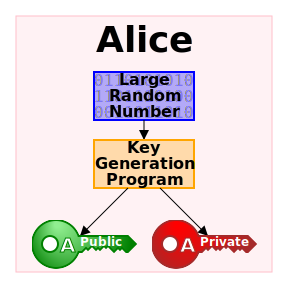
\includegraphics[width=6cm]{img/Public-key-crypto}\\
  &
  \begin{itemize}
    \item What about multiple devices?
  \end{itemize}
  \end{tabular}
  \end{table}
  \end{frame}

  \begin{frame}
  \frametitle{Keys derived from a password}
  \framesubtitle{Basic example}
  \framesubtitle{}
  $$ \text{DK}=\text{KDF}(\text{Key}, \text{Salt}, \text{Iterations}) $$
  \begin{table}
  \begin{tabular}{p{7cm}p{3cm}}
  Some functions for this are:
  \begin{itemize}
    \item PBKDF2
    \item scrypt
    \item bcrypt
    %\item What about multiple devices?
  \end{itemize}
  &
  \vspace{1.5cm}
  %\includegraphics[width=4cm]{../../presentacion/img/p2p-unstructured}\\
  \end{tabular}
  \end{table}
  \end{frame}


  \begin{frame}
  \frametitle{Probability of error}

      If $p$ represents the probability that a single node is malicious, and
      $N$ the total number of nodes in the DHT.\\

      With $p= 0.3$, for   
      $\frac{L}{2}$ consecutive nodes to be malicious in a leafset. The
probability is given by:

  \begin{equation} \label{eq:p_leafset}
    P= p^{\frac{L}{2}}
  \end{equation}

  \end{frame}

  \begin{frame}
  \frametitle{Trust in P2P networks}
  \framesubtitle{Probability of error}

  \begin{equation} \label{eq:p_leafset}
    P= p^{\frac{L}{2}}
  \end{equation}

  \begin{table}
    \centering
    \footnotesize
    \begin{tabular}{|c|c|c|}
      \cline{2-3}
      \multicolumn{1}{c|}{}&  \multicolumn{2}{c|}{\textbf{Probability to fail}} \\ \cline{2-3}
      \hline
      \textbf{Size of Trusted Set (L)} & \textbf{p = 0,3} & \textbf{p = 0,05} \\
      \hline \hline
      8 &  $0.0081$              & $6.25 \times 10^{-6}$  \\
      \hline
      16 & $6.56 \times 10^{-5}$ & $ 3.9 \times 10^{-11}$ \\
      \hline
      32 & $4.3 \times 10^{-9}$  & $ 1.52 \times 10^{-21} $  \\
      \hline
    \end{tabular}
    \caption{Probability of failure in a transaction that needs $L/2+1$
identical answers}
    \label{tab:p_leafset}
  \end{table}

  \end{frame}
  

\begin{frame}[allowframebreaks]
\frametitle{Methodology and Working plan}
\scriptsize
\noindent {\bf Stage I:} Problem definition
\begin{enumerate}
    \item Study of P2P network systems and P2P search and storage mechanisms.
          \emph{(August 2012)}
    \item Study the P2P networks capabilities to implement complex systems as
          seen in centralized systems.
          \emph{(September 2012 - November 2012)}
    \item Born of the idea.
          \emph{(December 2013)}
    \item Problem specification, hypothesis and project objectives.
          \emph{(February 2013)}
\end{enumerate}

\noindent {\bf Stage II:} P2P Systems definition
\begin{enumerate}
    \item State of the art of P2P network systems and P2P search and storage mechanisms.
          \emph{(May 2013)}
    \item State of the art of building of trust between nodes in P2P networks.
          \emph{(April 2013 - June 2013)}
    \item State of the art of user identification schemes in P2P networks and
          how to secure the different system protocols.
          \emph{(July 2013)}
\end{enumerate}

\noindent {\bf Stage III:} Solution proposal
\begin{enumerate}
    \item User identification system design for structured P2P networks.
          \emph{(August 2013 - September 2013)}
    \item Theoretic evaluation of the user identification proposal.
          \emph{(October 2013)}
    \item Final thesis report development.
          \emph{(November 2013 - January 2013 2013)}
    \item Paper development.
          \emph{(February 2014)}
\end{enumerate}
\normalsize
\end{frame}

  
\end{document}
